\documentclass[12pt, oneside]{article}
\usepackage[letterpaper, margin=1in]{geometry}
\usepackage[english]{babel}
\usepackage[utf8]{inputenc}
\usepackage{amsmath}
\usepackage{amsfonts}
\usepackage{amssymb}
\usepackage{tikz}
\usepackage{tkz-fct}

\usepackage{fancyhdr}
\pagestyle{fancy}
\fancyhf{}
\rhead{\thepage \\Name: \hspace{1.5in}.\\}
\lhead{BECA / Dr. Huson / 11.1 IB Math SL \\* 4 June 2018 \\* \textbf{Final Exam}}

\vspace{1cm}

\renewcommand{\headrulewidth}{0pt}

\title{Problem set template}
\author{Chris Huson}
\date{June 2018}

\begin{document}
%\maketitle

\subsubsection*{\\* \textnormal{Answer in pen. Show work. Graph carefully using pencil.}}

\begin{enumerate}
\item Given a loan or investment there are certain values to substitute into the appropriate formula. Assume\\[5pt]
\quad Principal amount invested, $P_0= \$1,000$\\[5pt]
\quad Interest rate, $r=5\% = 0.05$\\[5pt]
\quad Time, $t=5$ years \\[5pt]
\quad Compounding periods per year, $n=12$\\[15pt]
For each interest rate convention below, first write the formula, then substitute the values, finally, write down the final balance (use your calculator). 

\begin{enumerate}
    \item Continuous interest \\[1.25in]
    \item Monthly compounded interest \\[1.5in]
\end{enumerate}

\item Explain how $\displaystyle \left(2^{\frac{1}{5}} \right)^3$ can be written as the equivalent radical expression $\sqrt[5]8$. %Alg2 Regents Aug2016

\newpage
\item For each polynomial graph, state 
\begin{enumerate}
\item its degree,
\item how many distinct zeros it has, and
\item the sign of its leading coefficient.
\end{enumerate}

    \begin{tikzpicture}[scale=1.8/4]
    %\draw[step=1cm,gray,very thin] (-7,-7) grid (7,7);
    \draw[thick,<->] (-7.5,0) -- (7.5,0) node[anchor=north west] {\textbf{x}};
    \draw[thick,<->] (0,-5.5) -- (0,7.5) node[anchor=south east] {\textbf{y}};
    %\foreach \x in {-6, -4, -2, 2, 4, 6} \draw (\x cm,1pt) -- (\x cm,-1pt) node[anchor=north] {$\x$};
    %\foreach \y in {5} \draw (1pt,\y cm) -- (-1pt,\y cm) node[anchor=east] {50}; %{$\y$};
    \tkzInit[xmin=-6,xmax=6,ymin=-5,ymax=7,ystep=1]   
    \tkzFct[color=black,thick,<->,domain = -3.3:5.2] {0.05*(x*x*x*x-3*x*x*x-9*x*x+10*x+20)};
    \end{tikzpicture}
    \begin{tikzpicture}[scale=1.8/4]
    %\draw[step=1cm,gray,very thin] (-7,-7) grid (7,7);
    \draw[thick,<->] (-7.5,0) -- (7.5,0) node[anchor=north west] {\textbf{x}};
    \draw[thick,<->] (0,-5.5) -- (0,7.5) node[anchor=south east] {\textbf{y}};
    %\foreach \x in {-6, -4, -2, 2, 4, 6} \draw (\x cm,1pt) -- (\x cm,-1pt) node[anchor=north] {$\x$};
    %\foreach \y in {5} \draw (1pt,\y cm) -- (-1pt,\y cm) node[anchor=east] {50}; %{$\y$};
    \tkzInit[xmin=-6,xmax=6,ymin=-5,ymax=7,ystep=1]   
    \tkzFct[color=black,thick,<->,domain = -4.3:5.0] {-0.1*(x+3)*(x)*(x-4)};
    \end{tikzpicture}


\item Given a circle with radius of one, centered on the origin. An angle with measure $60^\circ$ is placed in standard position, with point $A$, the intersection of the circle and angle leg.
\begin{center}
\begin{tikzpicture}[scale=2.5]
  \draw[font=\scriptsize]
    (-1.2, 0) -- (1.2, 0)
    (0, -1.1) -- (0, 1.1)
    (0, 0) -- (0.5, .866) node[above right] {$\displaystyle A=\large{(} \qquad, \qquad \large{)}$}
    (0, 0) circle[radius=1]
    (-1, 0) node[below left] {$(-1,0)$}
    (1, 0) node[above right] {$(1,0)$}
    (1.1, 0) node[below right] {$\large{x}$}
    ;
\end{tikzpicture}
\end{center}
\begin{enumerate}
    \item On the graph, write down the exact values of the ordered pair, $A$. ("exact" means a fraction, radical, or exact decimal value, not a rounded number)
    \item Write down the exact value of $\sin{60^\circ}$\\[0.25in]
    \item  Write down the exact value of $\cos{60^\circ}$\\[0.25in]
\end{enumerate}


\newpage

\item Given $i$ is the imaginary unit, simplify $(3-zi)^2$ to the form $a+bi$. \\[1.3in]%Alg2 Regents Jun2016

\item The polynomial $f(x)=2x^3-3x^2-14x$ is shown on the graph below.
\begin{center}
    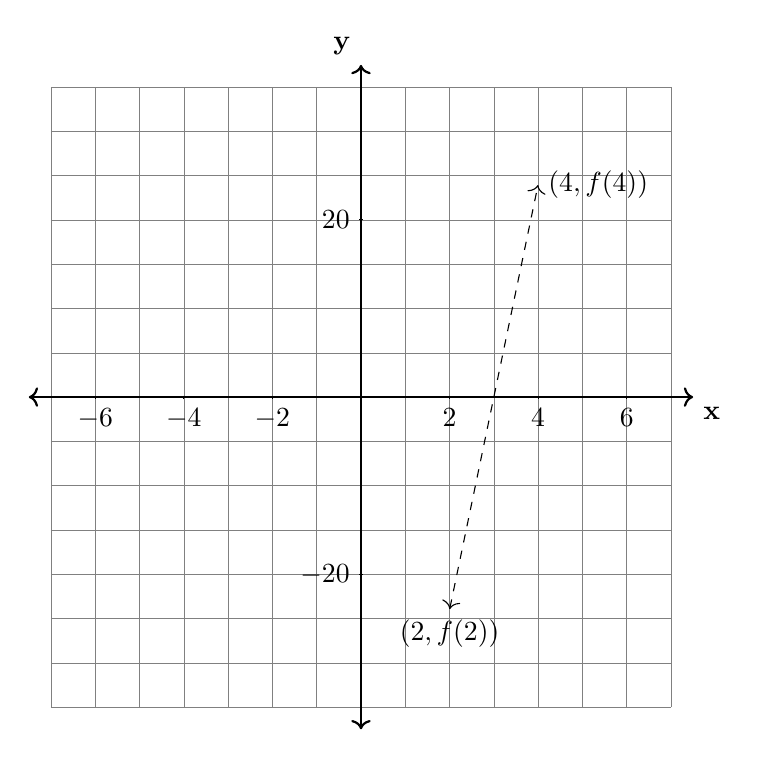
\begin{tikzpicture}[scale=2.25/4]
    \draw[step=1cm,gray,very thin] (-7,-7) grid (7,7);
    \draw[thick,<->] (-7.5,0) -- (7.5,0) node[anchor=north west] {\textbf{x}};
    \draw[thick,<->] (0,-7.5) -- (0,7.5) node[anchor=south east] {\textbf{y}};
    \foreach \x in {-6, -4, -2, 2, 4, 6} \draw (\x cm,1pt) -- (\x cm,-1pt) node[anchor=north] {$\x$};
    \foreach \y in {-4} \draw (1pt,\y cm) -- (-1pt,\y cm) node[anchor=east] {$-20$}; %{$\y$};
    \foreach \y in {4} \draw (1pt,\y cm) -- (-1pt,\y cm) node[anchor=east] {$20$};
    \tkzInit[xmin=-6,xmax=5,ymin=-5,ymax=7,ystep=1]   
    \tkzFct[color=black,thick,<->,domain = -2.5:4.1] {0.2*(2*x-7)*(x+2)*(x)};
    \draw [dashed] (2,-4.8) node[anchor=north] {$(2,f(2))$} -- (4,4.8) node[anchor=west] {$(4,f(4))$};
    \end{tikzpicture}
\end{center}
\begin{enumerate}
    \item The function can be written in factored form as $f(x)=(2x+k)(x+2)x$. Find $k$.\\[0.8in]
    \item What is the \emph{average rate of change} of the function between $x=2,4$.
\end{enumerate}


\newpage

\item Sketch a graph of a cubic polynomial with the following characteristics: 
\begin{itemize}
\item three positive, real zeros
\item as $x \rightarrow + \infty$, $f(x) \rightarrow + \infty$
\item as $x \rightarrow - \infty$, $f(x) \rightarrow - \infty$
\end{itemize}
\begin{center}
    \begin{tikzpicture}[scale=2/4]
    \draw[thick,<->] (-7.5,0) -- (7.5,0) node[anchor=north west] {\textbf{x}};
    \draw[thick,<->] (0,-7.5) -- (0,7.5) node[anchor=south east] {\textbf{y}};
    \end{tikzpicture}
\end{center} %Alg2 Regents Jun2016 MC

\item Given: $f(x)=3x^2- x + 2$ and $g(x)=3x+7$\\*[5pt]
Express $2 \bullet g(x) - f(x)$ as a polynomial in standard form. \\[3in] %Alg2 Regents Jan2018


\newpage
\item Two events $A$ and $B$ are such that $P(A)=0.2$ and $P(A \cup B) =0.5$. Given that $A$ and $B$ are mutually exclusive, find $P(B)$.\\[1.5in]

\item Find algebraically the zeros for  $g(x)=x^3+x^2-4x-4$.\\*[1.5in]
On the set of axes below, graph $y=g(x)$.
\begin{center}
    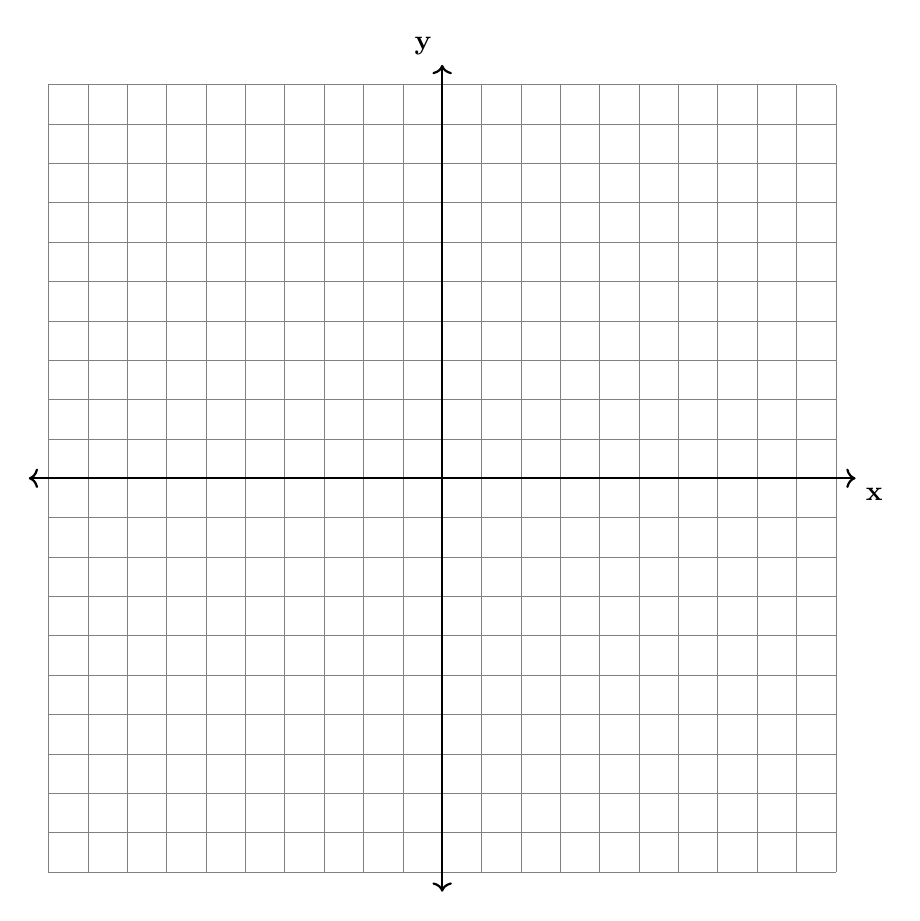
\begin{tikzpicture}[scale=2/4]
    \draw[step=1cm,gray,very thin] (-10,-10) grid (10,10);
    \draw[thick,<->] (-10.5,0) -- (10.5,0) node[anchor=north west] {\textbf{x}};
    \draw[thick,<->] (0,-10.5) -- (0,10.5) node[anchor=south east] {\textbf{y}};
    %\foreach \x in {-6, -4, -2, 2, 4, 6} \draw (\x cm,1pt) -- (\x cm,-1pt) node[anchor=north] {$\x$};
    %\foreach \y in {5} \draw (1pt,\y cm) -- (-1pt,\y cm) node[anchor=east] {50};
    %\foreach \y in {-5} \draw (1pt,\y cm) -- (-1pt,\y cm) node[anchor=east] {-50};    \tkzInit[xmin=-5,xmax=5,ymin=-7,ymax=7,ystep=1]
%    \tkzFct[color=black,thick,<->,domain = -3.4:7] {0.1*(x*x-4)*(x-5)};
    \end{tikzpicture}
\end{center} %Alg2 Regents Aug2016


\newpage
\item Express $2yi^3(xi-3)$ as a complex number in the form $a+bi$, $a,b \in \mathbb{R}$. \\[1.5in]

\item Write $\sqrt[4]x \cdot \sqrt{x}$ as a single term with a rational exponent. %Alg2 Regents Jun2017
\\*[1.5in]

\item Given events $A$ and $B$, such that $\mathrm \mathrm P(A)=0.6, \mathrm P(B)=0.5$, and $\mathrm P(A \cup B) =0.8$, determine whether $A$ and $B$ are dependent or independent. Justify your answer.\\[1.5in]

\item The function below models the average price of gas in a small town since January 1st.
\[G(t)=-0.006t^4 + 0.0823t^3 - 0.6t^2 +1.16t+3.2 \text{, where } 0 \leq t \leq 10.\]
If $G(t)$ is the average price of gas in dollars and $t$ represents the time in months since January 1st, the absolute maximum $G(t)$ reaches over the given domain is about what value, to the nearest cent? %Solution 3.86 Alg2 Regents Jan2018

\newpage

\item Researchers in a local area found that the population of rabbits with an initial population of 25 grew continuously at the rate of 4\% per month. The fox population had an initial value of 35 and grew continuously at the rate of 2\% per month.
\begin{enumerate}
    \item Write an expression representing the population of rabbits as a function of time $t$ in months.\\[1in] 
    \item Find the number of rabbits after 7 months, rounded to an integer.\\[2in] 
    \item Find, to the \emph{nearest tenth of a month}, how long it takes for the population of rabbits and foxes to be equal.
\end{enumerate} %Alg2 Regents Jan2018

\newpage
\item Consider the function $h(x) = 2\sin(3x) + 1$ and the function $q$ represented in the table below.\\*
\begin{center}
\begin{tabular}{|c|c|}
    \hline 
    $\boldsymbol{x}$ & $\boldsymbol{q(x)}$\\ 
    \hline 
    -2 & -8 \\ 
    \hline 
    -1 & 0 \\ 
    \hline 
    0 & 0 \\ 
    \hline 
    1 & -2 \\ 
    \hline 
    2 & 0 \\ 
    \hline 
\end{tabular}\\*[5pt]
\end{center}
Determine which function has the \emph{smaller} minimum value for the domain $[-2,2]$. Justify your answer. \\[2in]%Alg2 Regents Jan2018

\item A study was designed to test the effectiveness of a new drug. Half of the volunteers received the drug. The other half received a sugar pill. The probability of a volunteer receiving the drug and getting well was 40\%. What is the probability of a volunteer getting well, given that the volunteer received the drug? %Alg2 Regents Aug2017


\newpage
\item Jim is looking to buy a vacation home for \$165,000 near his favorite southern beach. The formula to compute a mortgage payment, $M$, is $\displaystyle M=P \cdot \frac{r(1+r)^N}{(1+r)^N-1}$ where $P$ is the principal amount of the loan, $r$ is the monthly interest rate, and $N$ is the number of monthly payments. Jim’s bank offers a monthly interest rate of 0.5\% for a 15-year mortgage.\\*[5pt]
With no down payment, determine Jim’s mortgage payment, rounded to the nearest dollar.\\*[3in]
Algebraically determine and state the down payment, rounded to the \emph{nearest dollar}, that Jim needs to make in order for his mortgage payment to be \$1250.
 %Alg2 Regents Jun2017 multiple choice

\newpage
\item The $x$-value of which function's $x$-intercept is larger, $f$ or $h$? Justify your answer. \[f(x)=\log (x-4) \]
\begin{tabular}{|c|c|}
\hline 
x & h(x)\\ 
\hline 
$-1$ & 6 \\ 
\hline 
0 & 4 \\ 
\hline 
1 & 2 \\ 
\hline 
2 & 0 \\ 
\hline 
3 & $-2$ \\ 
\hline 
\end{tabular}\\[2in] %Alg2 Regents Aug2016

\item Data collected about jogging from students with two older siblings are shown in the table below.\\*[5pt]
\begin{tabular}{|c|c|c|c|}
\hline 
& Neither Sibling & One Sibling & Both Siblings\\ 
& Jogs & Jogs & Jogs\\\hline 
Student Does Not Jog & 1168 & 1823 & 1380 \\ 
\hline 
Student Jogs & 188 & 416 & 400 \\ 
\hline 
\end{tabular}\\*[5pt]
Using these data, determine whether a student with two older siblings is more likely to jog if one sibling jogs or if \emph{neither} sibling jogs. Justify your answer. %Alg2 Regents Jun2017



\newpage
\item On the axes below, graph one cycle of a cosine function with amplitude 3, period $\displaystyle \frac{\pi}{2}$, midline $y=-1$, and passing through the point $(0,2)$.
\begin{center}
    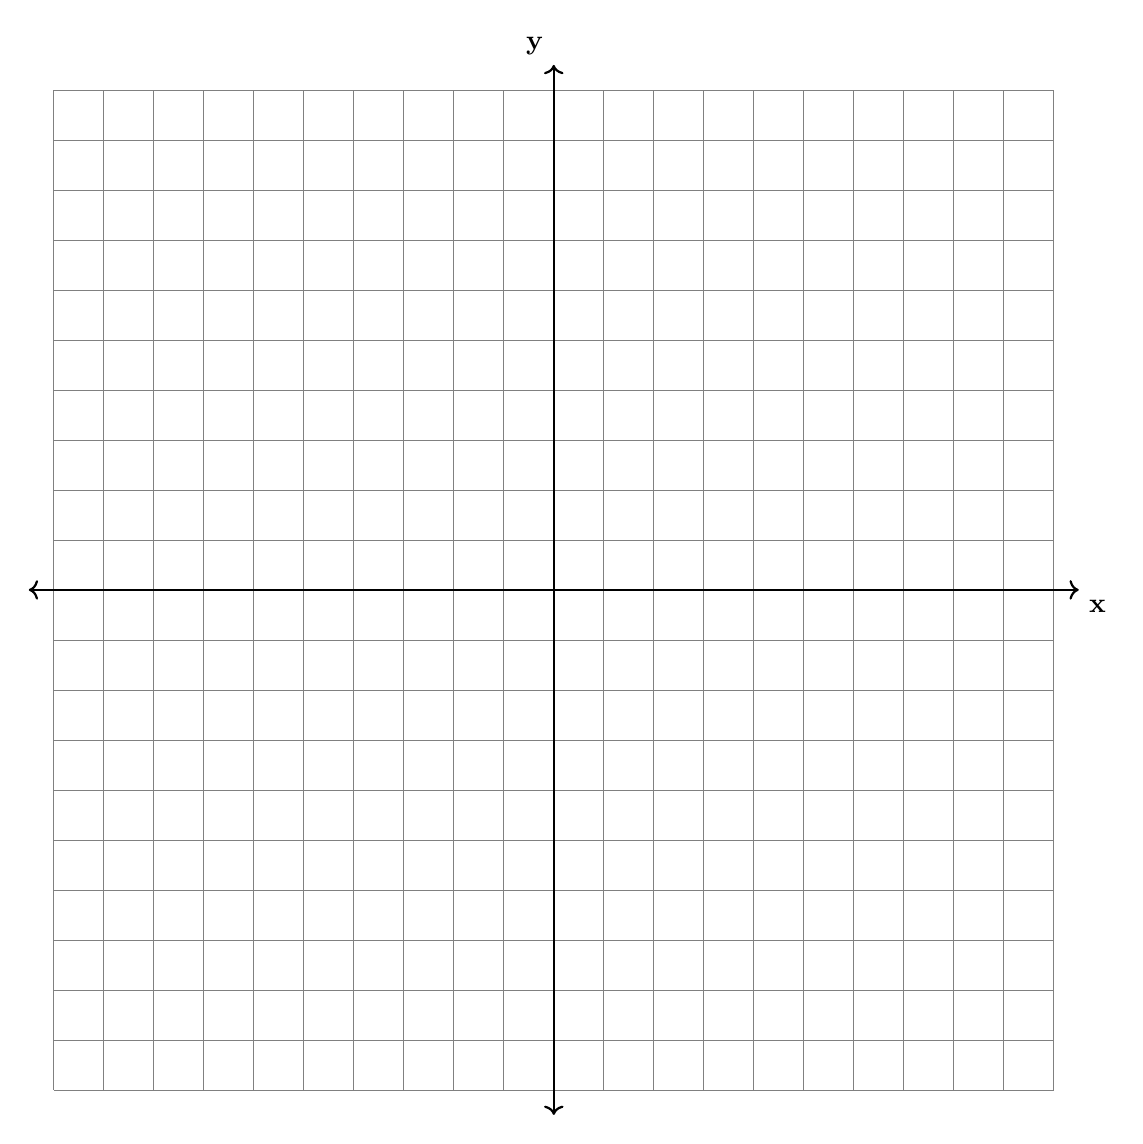
\begin{tikzpicture}[scale=2.54/4]
    \draw[step=1cm,gray,very thin] (-10,-10) grid (10,10);
    \draw[thick,<->] (-10.5,0) -- (10.5,0) node[anchor=north west] {\textbf{x}};
    \draw[thick,<->] (0,-10.5) -- (0,10.5) node[anchor=south east] {\textbf{y}};
    %\foreach \x in {-6, -4, -2, 2, 4, 6} \draw (\x cm,1pt) -- (\x cm,-1pt) node[anchor=north] {$\x$};
    %\foreach \y in {5} \draw (1pt,\y cm) -- (-1pt,\y cm) node[anchor=east] {50};
    %\foreach \y in {-5} \draw (1pt,\y cm) -- (-1pt,\y cm) node[anchor=east] {-50};    \tkzInit[xmin=-5,xmax=5,ymin=-7,ymax=7,ystep=1]
%    \tkzFct[color=black,thick,<->,domain = -3.4:7] {0.1*(x*x-4)*(x-5)};
    \end{tikzpicture} 
\end{center} %Jun2016 Regents FR

\newpage

\item Graph $y= \log_2(x+3)-5$ on the set of axes below. Use an appropriate scale to include both intercepts.
\begin{center}
    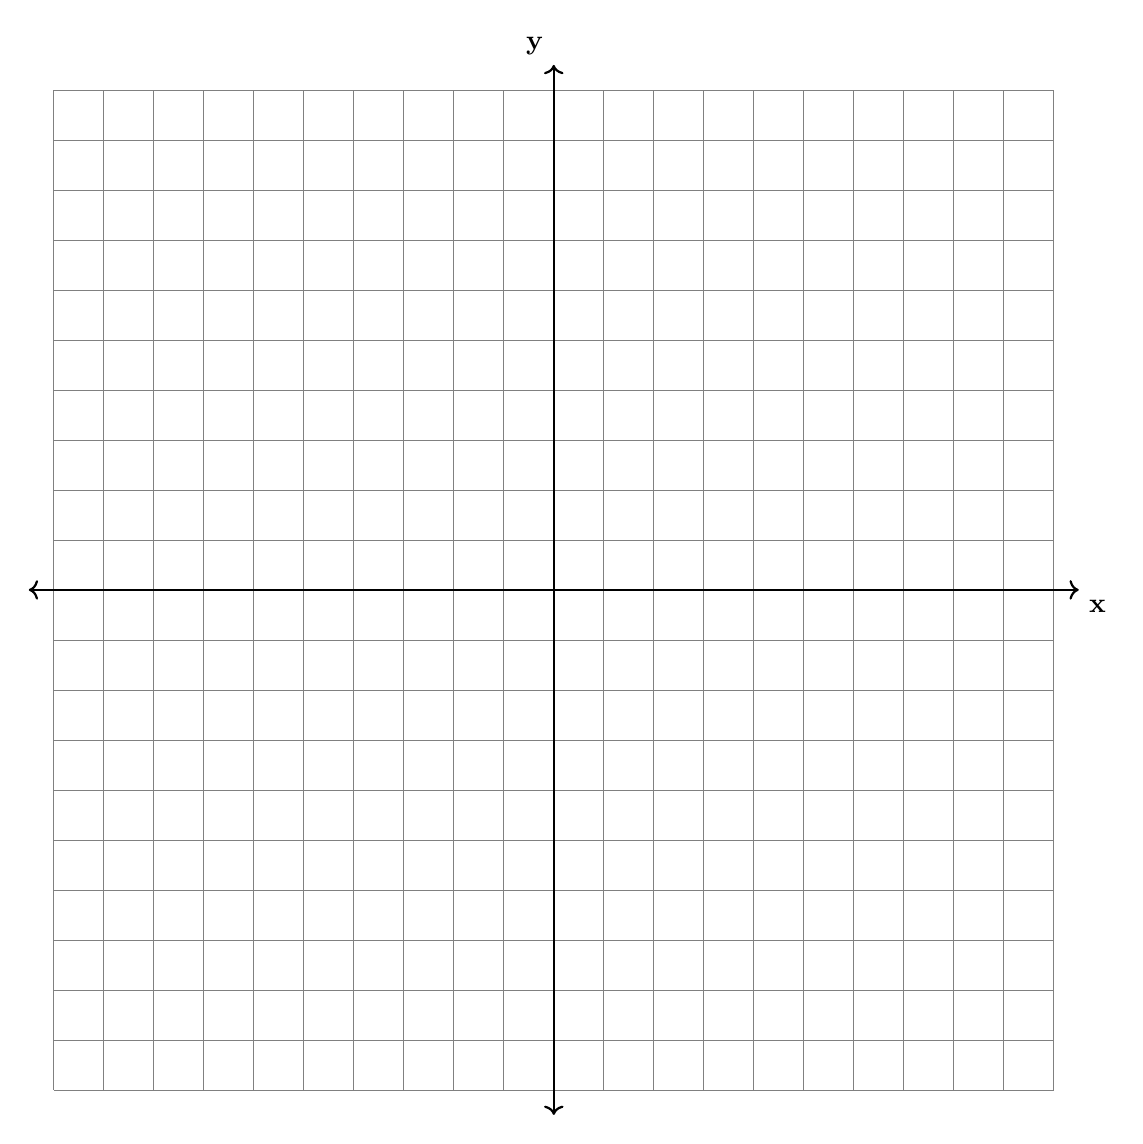
\begin{tikzpicture}[scale=2.54/4]
    \draw[step=1cm,gray,very thin] (-10,-10) grid (10,10);
    \draw[thick,<->] (-10.5,0) -- (10.5,0) node[anchor=north west] {\textbf{x}};
    \draw[thick,<->] (0,-10.5) -- (0,10.5) node[anchor=south east] {\textbf{y}};
%    \foreach \x in {-2, 2} \draw (\x cm,1pt) -- (\x cm,-1pt) node[anchor=north] {$\x$};
%    \foreach \y in {5} \draw (1pt,\y cm) -- (-1pt,\y cm) node[anchor=east] {50}; %{$\y$};
%    \tkzInit[xmin=-5,xmax=5,ymin=-7,ymax=7,ystep=1]   
%    \tkzFct[color=black,thick,<->,domain = -4.4:3.6] {0.1*(x+4)*x*x*(x-3)};
    \end{tikzpicture}
\end{center}

Describe the behavior of the given function as $x$ approaches $-3$ and as $x$ approaches positive infinity. %Alg2 Regents Jun2017 


\end{enumerate}
\end{document}


\item The value of a certain small passenger car based on its use in years is modeled by $V(t) =28482.698(0.684)^t$, where $V(t)$ is the value in dollars and $t$ is the time in years. Zach had to take out a loan to purchase the small passenger car. The function $Z(t)=22151.327(0.778)^t$, where $Z(t)$ is measured in dollars, and $t$ is the time in years, models the unpaid amount of Zach’s loan over time.\\*[10pt]
Graph $V(t)$ and $Z(t)$ over the interval $0 \leq t \leq 5$, on the set of axes below.
\begin{center}
    
\begin{tikzpicture}
    \draw[step=0.25in,gray,very thin] (0,0) grid (12.7,12.7);
    \draw[thick,->] (0,0) -- (13,0);% node[anchor=north west] {x};
    \draw[thick,->] (0,0) -- (0,13);% node[anchor=south east] {y};
    \end{tikzpicture}
\end{center}
State when $V(t)=Z(t)$, to the \emph{nearest hundredth}, and interpret its meaning in the context of the problem.\\*[10pt]
 %Alg2 Regents Aug2017
